\documentclass[12pt]{article}
\usepackage[utf8]{inputenc}
\usepackage[english]{babel}
\usepackage{listings}
\usepackage{tikz}
\usepackage{amsmath,amssymb}
\usepackage{subcaption}

\newcommand{\HRule}{\rule{\linewidth}{0.5mm}}

\begin{document}

\begin{center}
\textsc{\LARGE Principles of Computer System Design}\\[0.3cm] % Context
\HRule \\[0.4cm]
{ \huge \bfseries Assignment 4}
\HRule \\[0.4cm]
\large
Johannes de Fine Licht
\\Philip Graae
\\Ola Rønning
\\\today
\end{center}

\section*{Question 1: Reliability}

The two networks discussed below are shown in figure~\ref{fig:networks}.

\subsection*{1.}

For the daisy chain to connect all the buildings, both links must be active. Links have the probability of failing $p$, resulting in the added probability of failure $p_\text{daisy} = p + p - p\cdot p = 2p - p^2$.

\subsection*{2.}

For the fully connected network to fail, any two links would have to fail. This is the probability that any one link of the three links will fail, followed by the probability that any one of the remaining two links will fail. The event of a link failing is denoted as $A$, $B$ and $C$ in the below:

\begin{align*}
  P(((A\cup B)\cup C)\cap P(A\cup B)) = ((P(A) + P(B) - P(A\cap B)) \\
  \cap P(C)) \cup (P(A) + P(B) - P(A\cap B)) \\
  = (P(A) + P(B) - P(A\cap B) + P(C) + P(C) \cdot (P(A) + P(B) - P(A\cap B))) \\
  \cap (P(A) + P(B) - P(A\cap B)) \\ \Rightarrow
  p_{\text{full}} = (p + p - p^2 + p + p\cdot(p + p - p^2)) \cdot (p + p - p^2)\\
  = p^5 - 3p^4 - p^3 + 6p^2
\end{align*}

\subsection*{3.}

Probabilities of failure for the networks are now $p_{\text{daisy}} = 10^{-6}$ and $p_{\text{full}} = 10^{-4}$. \\
Based on the expressions derived above, this results in the probabilities:

\begin{align*}
  p_{\text{daisy}} = 2\cdot10^{-6} - 10^{-6\cdot2} \approx 2\cdot10^{-6} \\
  p_{\text{full}} = (10^{-4})^5 - 3(10^{-4})^4 - (10^{-4})^3 + 6(10^{-4})^2 \\
  = 10^{-20} - 3\cdot10^{-16} - 10^{-12} + 6\cdot10^{-8} \approx 6\cdot10^{-8}
\end{align*}

Even though the probability of a single link failing in the daisy network as compared to the full network is a hundred times lower, the more failure-tolerant design of the full network makes it the most reliable.

\subsection*{Assumptions}

In the above it has been assumed that:
\begin{itemize}
  \item Failures of different links are uncorrelated. In real-world scenarios, the source of a failure can often affect multiple components (lacking dissipation of heat, power outage, meteor strikes).
  \item The probability of $p$ is a \emph{probability of failure per unit of measurement}, where the unit of measurement can be a metric such as time or iterations. In the above the probability is assumed to be constant, while in normal hardware, the probability of failure typically is not constant in time/iterations.
\end{itemize}

\begin{figure}
\begin{subfigure}{.5\textwidth}
\centering
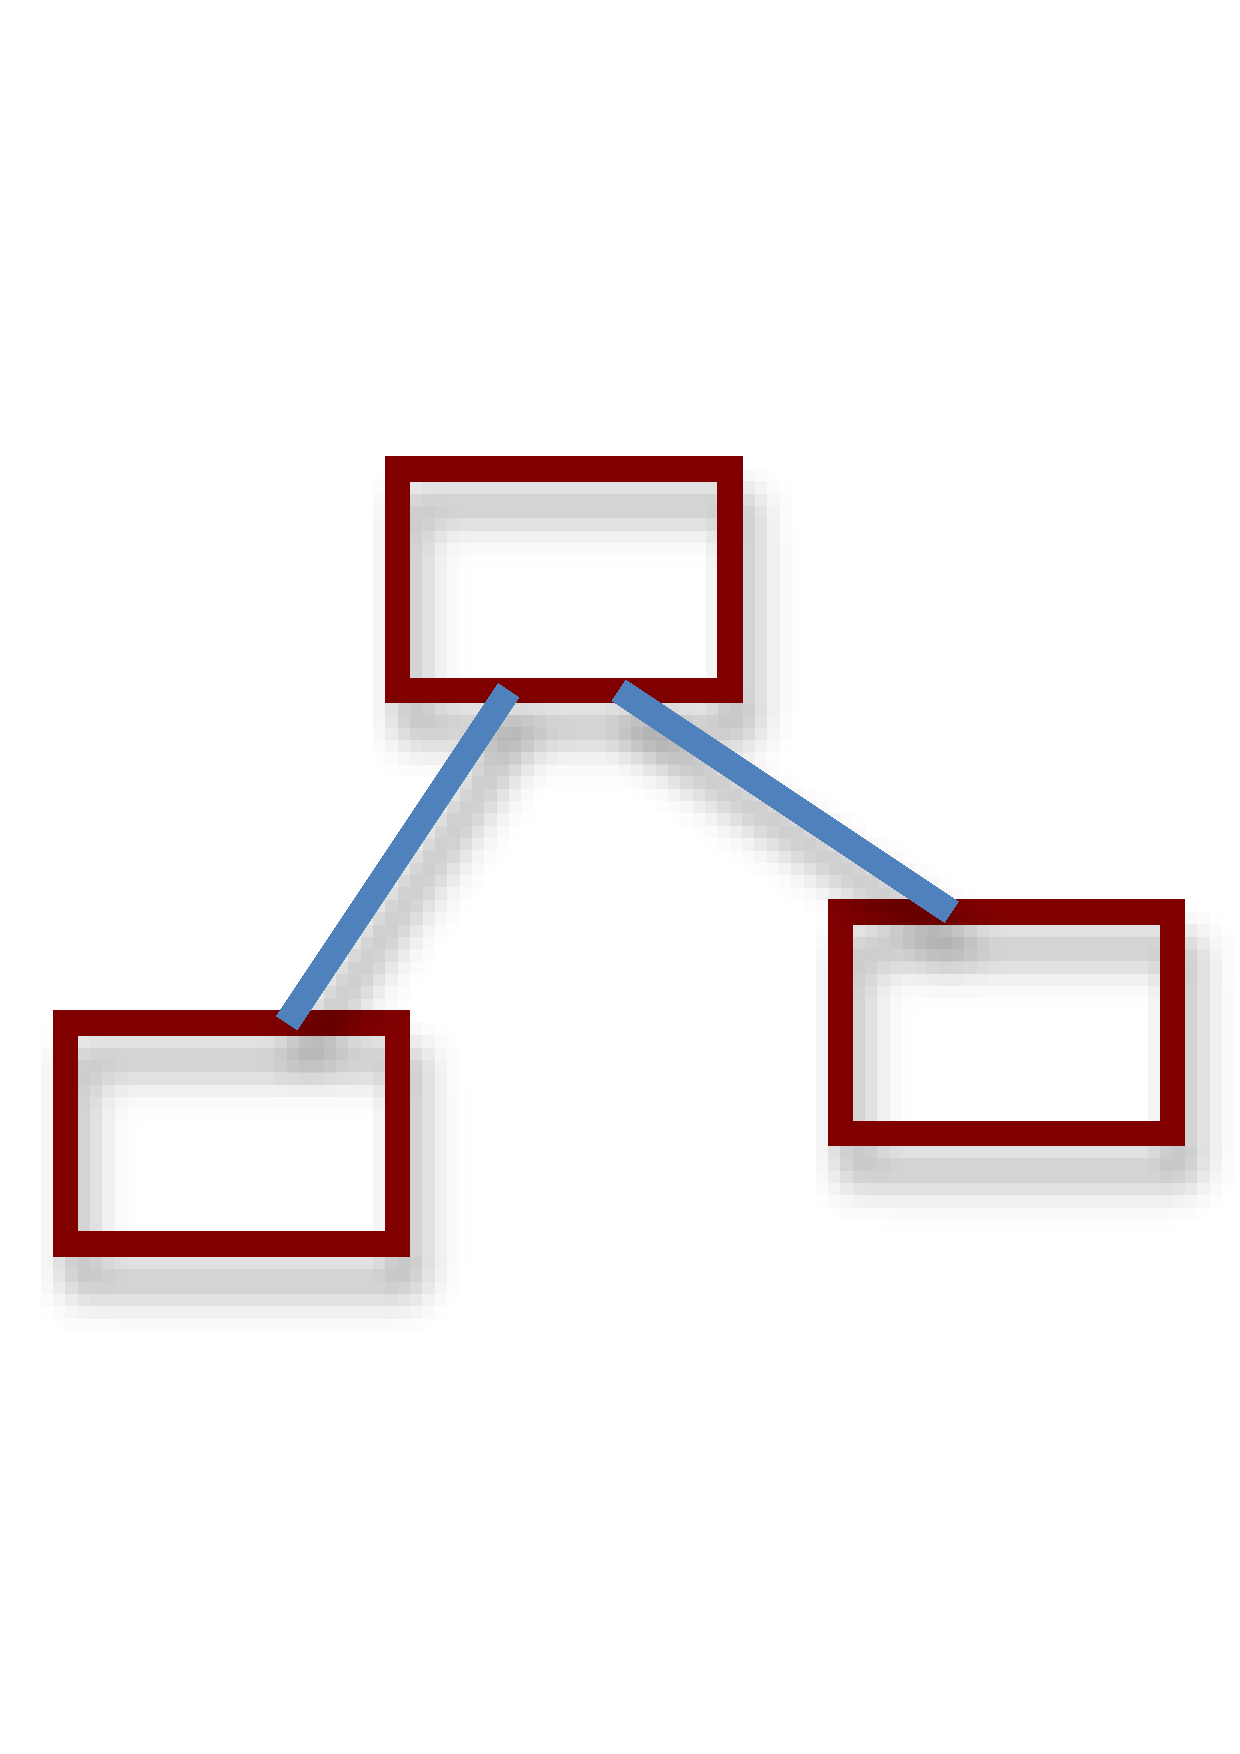
\includegraphics[width=.5\textwidth]{daisychain.pdf}
\caption{Daisy chain network.}
\end{subfigure}
\begin{subfigure}{0.5\textwidth}
\centering
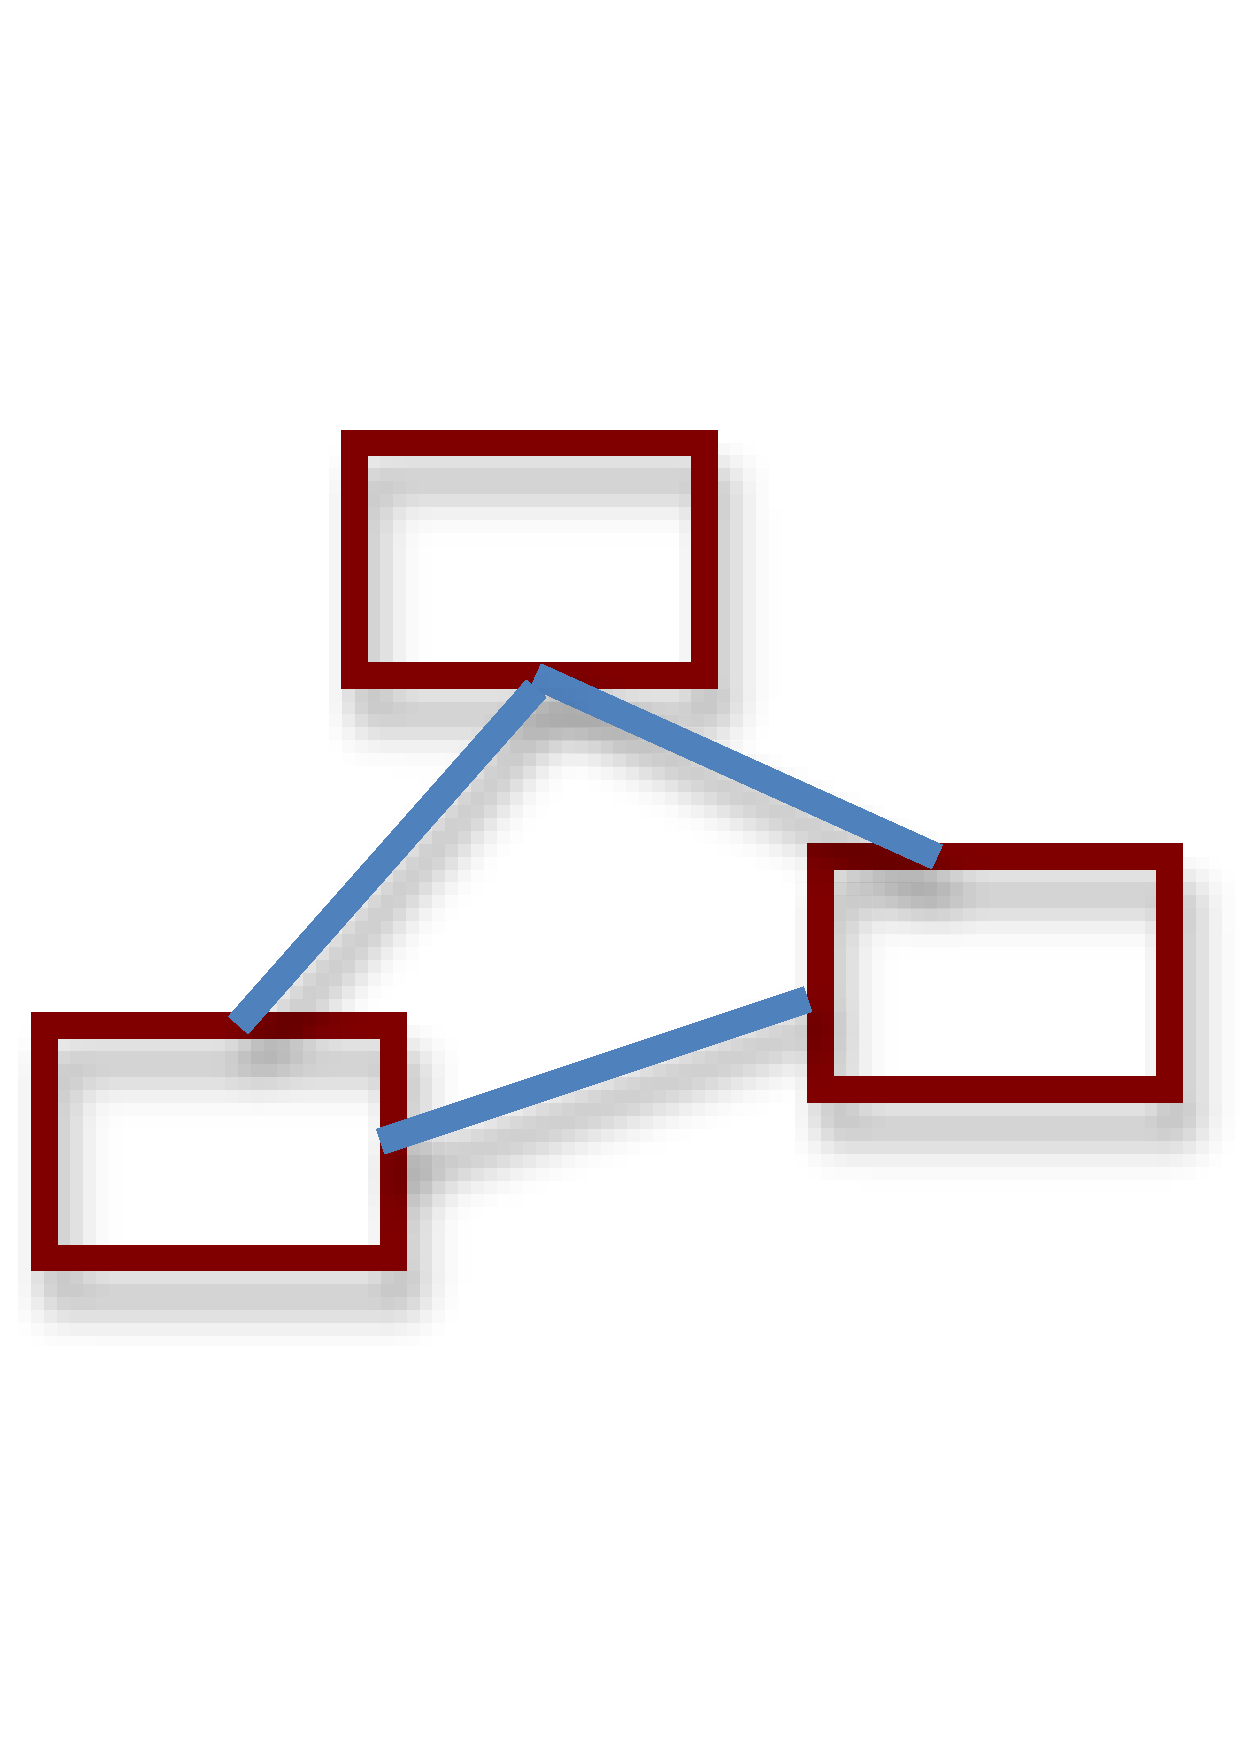
\includegraphics[width=.5\textwidth]{fullyconnected.pdf}
\caption{Fully connected network.}
\end{subfigure}
\caption{The two network models described in Question 1.}
\label{fig:networks}
\end{figure}

\section*{Question 2: Distributed Coordination}

For a two phase commit protocol, there is a risk of indefinite blocking if the coordinator and a participant both experience failure. This can occur after the voting phase, as the other nodes will not know whether the coordinator had already sent a commit or abort message to the crashed participant, and as such cannot proceed before receiving communication from the failed nodes. \\
For the three phase commit, the nodes first enter a \emph{preCommit} stage, then notify the coordinator that they are ready to commit. The coordinator will wait for acknowledgements from all nodes before sending the \emph{doCommit} message. If the coordinator and a participant fail at this stage, the other nodes will know and agree that both failed nodes were ready and had acknowledged the commit, resolving ambiguity concerning the state of the system which would otherwise requiring blocking following a two phase commit protocol.

\end{document}
